\section{Algoritmo Exacto}


\subsection{Algoritmo}
Antes de desarrollar la explicaci\'on, definimos algunos elementos que utilizaremos luego.
Sean G = (V, E$_G$), H = (V, E$_H$) dos grafos con V el mismo conjunto de nodos, y sea $n$  = $|$V$|$. 
Consideramos que los nodos de V se encuentran numerados de alguna manera con los n\'umeros de 1 a n.
Sean los n colores representados por el conjunto C = \{1, 2, ..., n\}; un coloreo ser\'a representado por una lista $f$ de n valores, cada uno de ellos pertenenciente al conjunto C, donde el nodo $i$ es pintado con el color en la posici\'on \textsl{f}$_i$.
Buscamos desarrollar un algortimo exacto que nos permita encontrar alg\'un coloreo \textsl{f} de G que use los colores de C, tal que el impacto (tal como se define en el enunciado) de \textsl{f} en H sea m\'aximo. 

La idea general del algoritmo es simple: generar todos los coloreos del grafo G, y por cada uno que sea legal, calcular el impacto en H y guardar aquel con el que el valor obtenido sea m\'aximo. 

Para genererar todos los coloreos posibles, vamos a partir de la siguiente funci\'on recursiva:

\begin{algorithm}[H]
\caption{} 
\begin{codebox}
\Procname{$\proc{coloreos}(nodo, coloreo)$}
\li \If \textit{nodo} $\leq$ \textsc{length}(\textit{coloreo}) \Do
\li 		\textsl{hacer algo con el coloreo}		
		\End
\li	\Else \Do
\li			\For color \textbf{in} Colores \Do	
\li					\textit{coloreo}[\textit{nodo}] = color
\li					\textsc{coloreos}(nodo+1, coloreo)	
				\End
		\End
\End
\end{codebox}
\end{algorithm}

Esta funci\'on genera todos las combinaciones posibles de los colores de C (\textsl{Colores}) en los nodos de G.
Sin embargo, \'esta es una tarea muy costosa, pues la cantidad de resultados posibles es de orden exponencial. Por ejemplo, si el grafo tiene n nodos, obtendr\'iamos al menos $n!$ coloreos: podr\'iamos colorear cada nodo de un color diferente, y despu\'es permutar los colores entre todos lo nodos. 
M\'as all\'a de esto, dadas las caracter\'isticas del problema planteado, veremos algunos recursos que nos permitiran reducir dr\'asticamente la cantidad de casos a analizar.


En primer lugar observamos que, para un grafo G dado, solo nos interesa analizar los coloreos que son legales (es decir, aquellos en los que si dos nodos son adyacentes, entonces est\'an pintados de colores distintos). Esto nos da una pauta sobre como aplicar podas a medida que vamos generando los coloreos: al pintar un nodo i (es decir, elegir un color para el posici\'on i del coloreo), utilizaremos solo los colores que produzcan un coloreo legal hasta ese momento.

Por ejemplo, en la figura \ref{fig:ejemploSoloColoreosNoValidos} mostramos dos pasos en la generaci\'on de un coloreo para un grafo de 5 nodos. Podemos ver que si tenemos el nodo 2 pintado de color negro, al pintar el nodo 3 tambi\'en de color negro obtendremos un coloreo ilegal para cualquier otra combinaci\'on de colores en los nodos siguientes. 

\begin{figure}[H]
	\centering
	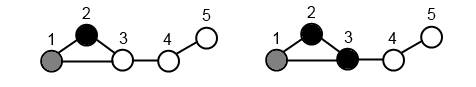
\includegraphics[scale=1]{ejemplo-coloreos-no-validos.png}
\caption{Ejemplo de coloreo de un nodo que lleva a coloreos ilegales.}
\label{fig:ejemploSoloColoreosNoValidos}
\end{figure}

Por lo tanto, podemos aplicar una una poda considerando solamente los colores que sean legales con respecto a los de los nodos pintados con anterioridad:

\begin{algorithm}[H]
\caption{} 
\begin{codebox}
\Procname{$\proc{coloreos}(nodo, coloreo)$}
\li \If \textit{nodo} $\leq$ \textsc{length}(\textit{coloreo}) \Do
\li 		\textsl{hacer algo con el coloreo}		
		\End
\li	\Else \Do
\li			\For color \textbf{in} Colores \Do
\li		 		\If color legal para el nodo \textsl{nodo}\Do	
\li					\textit{coloreo}[\textit{nodo}] = color
\li					\textsc{coloreos}(nodo+1, coloreo)	
					\End
				\End
		\End
\End
\end{codebox}
\end{algorithm}
 
Por otro lado, notamos que existen coloreos que son equivalentes (en el sentido en que uno puede obtenerse a partir del otro por medio de un renombramiento de sus colores), y por lo tanto, una vez analizado un caso, los dem\'as solo aportan informaci\'on redundante. 
Por ejemplo, supongamos que tenemos un grafo de 5 nodos 3-coloreable, y sean C = \{\textsl{gris} = 1, \textsl{rayado} = 2, \textsl{negro} = 3\} los colores. 
Dos coloreos v\'alidos son 1-2-3-1-2 y 2-1-3-2-1, como se muestra en la figura \textbf{\ref{fig:ejemploRepeticionColoreo}}. 
Sin embargo, f\'acilmente se ve que al intercambiar las etiquetas de los colores \textsl{1} y \textsl{2}, el primer coloreo puede transformase en el segundo, y el segundo puede transformase en el primero. 

\begin{figure}[H]
	\centering
	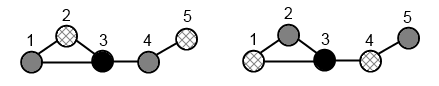
\includegraphics[scale=1]{ejemplo-mismos-coloreos.png}
\caption{Ejemplo de dos coloreos legales que resultan equivalentes.}
\label{fig:ejemploRepeticionColoreo}
\end{figure}


Recordemos que numeramos los nodos y los colores con los n\'umeros de 1 a n, y dejemos de lado, por el momento, la condici\'on de legalidad.
Definamos un conjunto de coloreos F donde cada coloreo f es un vector 
$$f = [f(1), ... , f(n)]$$


tal que, para cada uno, $f(v)$ cumple

\begin{itemize}
	\item $m$ es el m\'aximo en $f[1...v-1]$ (0, si $v-1 \leq 0$)
	\item $1 \leq f(v) \leq m+1$
\end{itemize}

Es decir, para pintar el nodo v, se usan $m+1$ maneras distintas, usando los colores ya usados, de 1,2...$m$ o un color nuevo, $m+1$.

\begin{figure}[H]
	\centering
	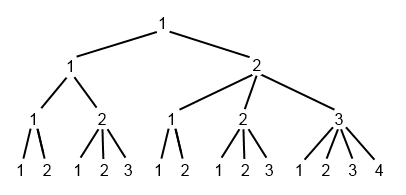
\includegraphics[scale=1]{ejemplo-coloreos-distintos.png}
\label{fig:ejemploColoreosDistintos}
\caption{Ejemplo de un conjunto de coloreos seg\'un la caracterizaci\'on dada. Cada camino desde la ra\'iz a una hoja es un coloreo. Por ejemplo, 1-1-1-1, 1-2-1-2 y 1-2-3-4.}
\end{figure}


Por la forma en que estan construidos, resulta que dos coloreos f y f' cualesquiera de F no son equivalentes. 
Adem\'as, cualquier otro coloreo que no est\'e en F es equivalente a uno que si lo est\'a.

Entonces, para evitar analizar mas de una vez coloreos equivalente, definimos una forma m\'as restrictiva para armar los coloreos basandonos en lo anteriormente expuesto.
El pseudoc\'odigo del algoritmo (ya considerando la selecci\'on del coloreo de m\'aximo impacto cada vez que completamos un coloreo) es el siguiente:

\begin{algorithm}[H]
\caption{} 
\begin{codebox}
\Procname{$\proc{colorear}(nodo i, grafo G, grafo H, coloreo, solucion)$}

\li \If $i \; \geq \; G.cantNodos$ \Comment{se pintaron todos los nodos de G} \Do
\li	$impacto$ $\gets$ impacto del coloreo en H
\li		\If $impacto\; > \; solucion.impacto$ \Do
\li			$solucion.impacto \gets impacto$
\li			$solucion.coloreo = coloreo$
			\End
	\End
\li \Else \Do
\li		$maxColor$ $\gets$ maximo color usado hasta el momento 	
\li		\For c \textbf{from} 1 \textbf{to} maxColor \Do
\li			\If es legal pintar el nodo $i$ de color c \Do
\li					$nuevoColoreo \; = \; coloreo$
\li         $nuevoColoreo[i] \gets c$
\li         $colorear(i+1, G, H, nuevoColoreo, solucion)$
             \End
         \End
\End
\end{codebox}
\end{algorithm}


La funci\'on que resolver\'a el problema planteado es

\begin{algorithm}[H]
\caption{} 
\begin{codebox}
\Procname{$\proc{maximoImpactoExacto}(Grafo$ G$, Grafo$ H$)$}
\li Sea $solucion$ un vector de n+1 elementos
\li Sea $coloreo$ un vector de n elementos
\li $solucion[0] \gets 0$
\li $coloreo[0] \gets 1$
\li $colorear(1,g,h,coloreo,solucion)$
\li	return $solucion$
\End
\end{codebox}
\end{algorithm}



\subsection{Análisis de complejidad}

\indent Al momento de hacer este análisis de complejidad se tuvieron en cuenta algunas consideraciones.\\
\indent En primer lugar, llamaremos $m$ al máximo entre la cantidad de aristas del grafo G y del grafo H  y $n$ a la cantidad de nodos de dichos grafos.\\
\indent En segundo lugar, en el análisis de complejidad de la función $colorear$ se definirá $k$ como la cantidad de nodos que quedan por pintar hasta ese paso de la recursión, en contraste con la implementación donde la recursión es , por así decirlo $hacia arriba$, significando esto que se inicia desde el primer nodo y se va hacia el último.\\

\indent Analicemos primero la función $colorear$. Como mencionamos anteriormente, consideraremos la recursión en la cantidad de nodos que quedan por colorear.

\indent El caso base será cuando no hayan más nodos por pintar. En dicho caso, el algoritmo simplemente calcula el impacto de dicho coloreo en el grafo H y en caso de ser el de máximo impacto hasta el momento se reemplaza la solución anterior por la nueva. Esto cuesta O(n+m), que es lo que cuesta calcular el impacto en H.\\
\indent Para el caso en el que la cantidad de nodos a pintar sea distinta de cero, el algoritmo calcula los posibles colores con los que pintar el nodo. Esto lo hace buscando cuál es el máximo color usado hasta el momento. El nuevo nodo podrá ser pintado de los colores usados anteriormente o del máximo color usado hasta el momento + 1, es decir pintándolo de un nuevo color. Esto se calcula en tiempo O(n).Luego se llamará a la función recursivamente una cantidad de veces igual al máximo color a utilizar. Ese valor se puede acotar para todos los casos por n-k+1.\\
\indent Además se chequea que agregar ese color genere un coloreo válido, y eso cuesta O(cantidad de vecinos del nodo), que lo podemos acotar por la cantidad de aristas de G, es decir O(m). Luego se hace la llamada recursiva para la instancia inmeditamente menor.\\
\indent Pasando en limpio, en el paso $k$ el algoritmo cuesta (n-k+1)*(n+m + T(k-1)).\\
\indent Es decir:\\

\indent T(0)=n+m\\
\indent T(k)=(n-k+1)*[(n+m)+ T(k-1)]\\

donde $k$ es la cantidad de nodos que quedan por pintar.\\


Veamos entonces cuánto cuesta pintar todos los nodos.\\
Basado en la definición que dimos antes, si tenemos que pintar todos los nodos, estamos en el caso T(n) = (n-n+1)*(n+m + T(n-1)).
Desarrollemos T(n):
\vspace{1em}

\begin{centering}
T(n)=(n-n+1)*(n+m + T(n-1))\\
= n+m + [2*(n+m) + 2*T(n-2)]\\
=(n+m)+2*(n+m) + 2*[3*(n+m)+ 3* T(n-3)]\\
=(n+m)+2*(n+m)+ 2*3*(n+m) + 2*3 T(n-3)\\
=(n+m)+2*(n+m)+ 2*3*(n+m) + 2*3*[4*(n+m)+4*T(n-4)]\\
=(n+m)+2*(n+m)+2*3*(n+m)+2*3*4*(n+m)+ 2*3*4*T(n-4)\\
...\\
=[ $\sum_{i=1}^{n} i! * (n+m) $] + n! * T(0) \\
=[ $\sum_{i=1}^{n} i! * (n+m) $] + n! * (n+m)\\
\end{centering}

\indent Es decir que $$T(n)= \left[ \sum_{i=1}^{n} i! * (n+m) \right] + n! * (n+m)$$\\

Conjeturamos entonces que T(n) es O($\sum_{i=1}^{n} i! * (n+m) $).
Veámoslo por inducción en la cantidad de nodos por pintar. 
Queremos ver que existe un $d \in \mathbb{R}_{> 0}$ y $n_{0}  \in \mathbb{N}$ tales que para todo $n \geq n_{0}$ vale que $T(n) \leq d * [\sum_{i=1}^{n} i! * (n+m)] $.

\begin{itemize}
	\item Caso base: n=1 
\begin{center}
T(1)= $\sum_{i=1}^{1} i! * (1+m)  1! * (1+m) $ = 2*1!*(1+m)\\
=2*(1+m) $\leq$ 2*  $\sum_{i=1}^{1} i! * (1+m)$ 
\end{center}

Es decir que alcanza con tomar $d=2$.

\item Paso inductivo: suponiendo que vale que $T(n-1) \leq d * [\sum_{i=1}^{n-1} i! * (n-1+m)] $ queremos ver que vale $T(n) \leq d * [\sum_{i=1}^{n} i! * (n+m)] $ 

\begin{center}

$T(n)=(n-n+1)*(n+m + T(n-1))= (n+m) + T(n-1) $\\

$\stackrel{HI}{\leq} n+m + d * [\sum_{i=1}^{n-1} i! * (n-1+m)] $

$\leq n+m + d * [\sum_{i=1}^{n-1} i! * (n+m)] $ \\

$\leq (n+m) *[ (d* \sum_{i=1}^{n-1} i!) + 1] $ \\

$\leq (n+m) *[ (d* \sum_{i=1}^{n-1} i!) + n!]$ \\

$\leq (n+m) *[ (d* \sum_{i=1}^{n} i!)] $\\

$\leq  d* \sum_{i=1}^{n} i!*(n+m)$\\

\end{center}

\indent que es lo que queríamos ver.\\
\end{itemize}

Por lo tanto, las complejidades son

\begin{itemize}
	\item \textsc{colorear}: O($\sum_{i=1}^{n} i! * (n+m) $)
	\item \textsc{maximoImpactoExacto}: O(n+1 + n + 1 + $\sum_{i=1}^{n} i! * (n+m) $) = O($\sum_{i=1}^{n} i! * (n+m) $)
\end{itemize}

\subsection{Experimentación y Resultados}

\quad Para realizar testeos y generar resultados lo más diversos posibles definimos 3 familias de grafos:

\begin{itemize}
\item \textbf{Grafos aleatorios:} \quad Primero creamos un grafo de la cantidad de vértices deseada pero sin aristas. Luego recorremos todos los nodos por orden de etiqueta. Por cada nodo, determinamos si esta conectado a cada uno de los otros nodos. Usamos la función \textit{rand()} de la Standar Library de $C++$ con una probabilidad del $ 30\div $ si de que esté unido a un nodo. 

 \quad Vimos que la probabilidad si es mayor se generan casi siempre grafos conexos. Como buscamos que sean lo más diversos posibles, nos pareció un valor razonable donde se generan diversas componentes conexas y hasta incluso grafos conexos.

\quad

\item \textbf{Grafos Estrella no uniformes (Star):} \quad Se parte un nodo central luego se le añaden 4 nodos a los cuales los consideremos externos. Se van a ir agregando nodos hasta la cantidad deseada. Un nodo que se agrega puede estar conectado con un nodo \textit{externo} o el nodo central. Si se agrega al nodo externo se considera como un nuevo nodo externo. Si se conecta con un nodo externo, éste deja de serlo y el nuevo nodo pasa a ser externo. 

\quad Así, todos los nodos menos el central tienen grado uno o dos. Si es externo grado 1, caso contrario 2. El grado del nodo interno varia con cada creación de grafo. La elección a qué nodo se uno se hace aleatoriamente usando la misma función mencionada para los grafos aleatorios.

\quad

\item \textbf{Grafos Web de 4 vértices (Red)\footnote{http://en.wikipedia.org/wiki/List\_of\_graphs}:} \quad estos grafos son un caso particular de grafos $ Web_{s t} $ que son t ciclos de s vértices cada uno conectados entre los ciclos un nodo con un solo nodo del ciclo aledaño. 
\end{itemize}

\quad

\quad \textbf{Aclaración Importante:} Vamos a trabajar con estas familias de grafos con el resto de las experimentaciones de este trabajo práctico. Los resultados (datos procesados y no procesados) de las experimentaciones se encuentran en la carpeta \textit{resultados}.

\quad 

\quad Se midieron los tiempos en corridas de  5 a 15 nodos con 50 repeticiones para cada cantidad de nodos.

\begin{figure}[H]
	\centering
	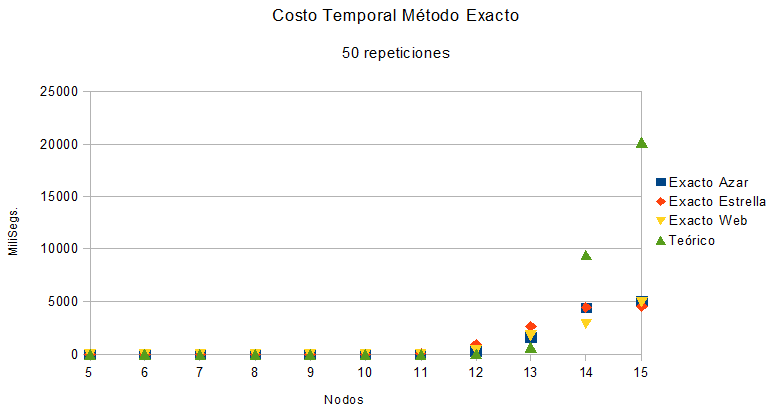
\includegraphics[scale=0.8]{timingExacto.png}
\caption{Costos}
\end{figure}

\quad Debido al gran costo computacional de este método no se puede experimentar con una mayor cantidad de nodos sin que tome una cantidad de tiempo considerable. Elegir esa cantidad nos permite realizar varias repeticiones para obtener resultados más fiables.

\quad Podemos observar que en este método no influye la diferencia entre las familias de grafos, tomando para cada uno el mismo costo temporal. 

\quad A partir del nodo 14 se ve claramente como la cota teórica sobrepasa a los resultados obtenidos. Éstos muestran una tendencia con una curvatura mucho menos pronunciada que la teórica.

\quad Las mediciones estan en milisegundos, por lo que son despreciables los resultados con pocos nodos que toman pocos milisegundos pero se ve que a medida que aumenta la cantidad de nodos aumenta considerablemente el costo temporal.

